% RSA-SHIELD — 10 pages, white, full-bleed content, larger fonts
% Team Aegis | Dr. Sachin Choudhary | Bennett University
% pdfLaTeX ×2

\documentclass[12pt,landscape]{article}

\usepackage[a4paper,left=0.75cm,right=0.75cm,top=0.45cm,bottom=0.75cm]{geometry}
\usepackage[T1]{fontenc}
\usepackage[utf8]{inputenc}
\usepackage{lmodern}
\usepackage{xcolor}
\usepackage{tikz}
\usepackage{enumitem}
\usepackage{fancyhdr}
\usepackage{hyperref}

\usetikzlibrary{arrows.meta,positioning}

\definecolor{ink}{HTML}{1A1F2E}
\definecolor{body}{HTML}{334155}
\definecolor{muted}{HTML}{64748B}
\definecolor{line}{HTML}{CBD5E1}
\definecolor{pane}{HTML}{F8FAFC}
\definecolor{pane2}{HTML}{EFF6FF}
\definecolor{cyan}{HTML}{0E7490}
\definecolor{violet}{HTML}{6D28D9}
\definecolor{amber}{HTML}{B45309}
\definecolor{crit}{HTML}{B91C1C}
\definecolor{ok}{HTML}{047857}

\pagecolor{white}
\color{ink}
\pagestyle{fancy}
\fancyhf{}
\renewcommand{\headrulewidth}{0pt}
\renewcommand{\footrulewidth}{0.45pt}
\renewcommand{\footrule}{\hbox to\headwidth{\color{line}\leaders\hrule height \footrulewidth\hfill}}
\fancyfoot[L]{\small\textcolor{muted}{RSA-SHIELD $\cdot$ Team Aegis}}
\fancyfoot[C]{\small\textcolor{muted}{Bennett University}}
\fancyfoot[R]{\small\textcolor{muted}{\thepage\,/\,10}}
\setlength{\parindent}{0pt}
\setlist[itemize]{leftmargin=1.1em,itemsep=3.5pt,topsep=2.5pt,parsep=0pt}
\setlist[enumerate]{leftmargin=1.2em,itemsep=3.5pt,topsep=2.5pt,parsep=0pt}

\newcommand{\slidetitle}[1]{{\LARGE\bfseries\color{ink}#1}\par\vspace{2pt}{\color{cyan}\hrule height 1.4pt}\vspace{6pt}}

% Stretch page to kill blank half-pages (leave room for footer)
\newenvironment{slidepage}{%
  \noindent\begin{minipage}[t][\dimexpr\textheight-0.35cm\relax][s]{\textwidth}%
}{\end{minipage}\newpage}

\tikzset{
  boxcyan/.style={draw=cyan, fill=pane2, rounded corners=2.5pt, text=ink,
    align=center, font=\small\sffamily\bfseries, inner sep=5pt, minimum height=0.82cm},
  boxvio/.style={draw=violet, fill=pane, rounded corners=2.5pt, text=ink,
    align=center, font=\small\sffamily\bfseries, inner sep=5pt, minimum height=0.82cm},
  boxamb/.style={draw=amber, fill=pane, rounded corners=2.5pt, text=ink,
    align=center, font=\small\sffamily\bfseries, inner sep=5pt, minimum height=0.82cm},
  boxred/.style={draw=crit, fill=pane, rounded corners=2.5pt, text=ink,
    align=center, font=\small\sffamily\bfseries, inner sep=5pt, minimum height=0.82cm},
  boxok/.style={draw=ok, fill=pane, rounded corners=2.5pt, text=ink,
    align=center, font=\small\sffamily\bfseries, inner sep=5pt, minimum height=0.82cm},
  boxmut/.style={draw=muted, fill=pane, rounded corners=2.5pt, text=ink,
    align=center, font=\small\sffamily\bfseries, inner sep=5pt, minimum height=0.82cm},
  arr/.style={-{Latex[length=2mm]}, draw=muted, line width=0.7pt}
}

\begin{document}

%% 1 COVER
\begin{slidepage}
{\color{cyan}\hrule height 3.2pt}\vspace{0.3cm}
{\normalsize\bfseries\color{cyan}COLLEGE PROJECT PRESENTATION $\cdot$ CYBERSECURITY / CRYPTOGRAPHY}\\[0.4em]
{\fontsize{32}{36}\selectfont\bfseries\color{ink}RSA-SHIELD}\\[0.25em]
{\Large\color{body}An Intelligent RSA Key Security Auditor for Legacy Critical Infrastructure}\\[0.25em]
{\normalsize\color{muted}Software auditing platform using established cryptography (RSA + Lenstra ECM) --- not a new cryptosystem.}
\vspace{\fill}

\begin{minipage}[t]{0.58\textwidth}
\fcolorbox{cyan}{pane}{\begin{minipage}[t]{0.96\textwidth}\vspace{6pt}
{\large\bfseries\color{cyan}Team Aegis}\\[0.45em]
{\normalsize
\begin{tabular}{@{}p{5.4cm}l@{}}
Nishant Agarwal & \texttt{S24CSEU1512}\\[0.2em]
Adarsh Agrahari & \texttt{S24CSEU1187}\\[0.2em]
Shubh Jadiya & \texttt{S24CSEU0530}\\
\end{tabular}}\\[0.45em]
{\normalsize Mentor: \textbf{Dr.\ Sachin Choudhary}\\[0.15em]
Institution: \textbf{Bennett University}}
\vspace{4pt}\end{minipage}}

\vspace{0.5cm}
{\Large\bfseries Project objective}\\[0.25em]
{\normalsize\color{body}Build a software-only cybersecurity platform that accepts RSA public keys/moduli, analyzes cryptographic properties, attempts mathematical factorization using Lenstra's Elliptic Curve Method (ECM) where appropriate, identifies suspicious or weak RSA configurations, and generates an understandable, evidence-tiered security assessment for authorized infrastructure owners.}

\vspace{0.4cm}
{\Large\bfseries Why it matters}\\[0.25em]
{\normalsize\color{body}Legacy SCADA/substation systems may still encrypt successfully while hiding weak key material. RSA-SHIELD helps owners move from simple key inventories to \textbf{mathematical assurance}---without claiming to invent RSA or ECM.}
\end{minipage}\hfill
\begin{minipage}[t]{0.38\textwidth}
\fcolorbox{cyan}{pane2}{\begin{minipage}[t]{0.94\textwidth}\vspace{8pt}\centering
{\Large\bfseries\color{cyan}$n = p \times q$}\\[0.5em]
{\normalsize\color{body}RSA security depends on secrecy of the primes behind the modulus.}\\[0.55em]
{\normalsize\bfseries Audit outcome tiers}\\[0.35em]
{\normalsize
\textcolor{crit}{\textbf{Factor Found}} --- hard evidence\\[0.25em]
\textcolor{amber}{\textbf{Suspicious}} --- heuristic warning\\[0.25em]
\textcolor{violet}{\textbf{Inconclusive}} --- no factor in budget\\[0.25em]
\textcolor{ok}{\textbf{No weakness}} by configured checks}\\[0.45em]
{\small\color{muted}Evidence is never confused with heuristics.}
\vspace{6pt}\end{minipage}}

\vspace{0.45cm}
\fcolorbox{violet}{pane}{\begin{minipage}[t]{0.94\textwidth}\vspace{6pt}
{\normalsize\bfseries\color{violet}Audience}\\[0.2em]
{\normalsize\color{body}Faculty, cybersecurity evaluators, technical judges, and software engineering reviewers.}
\vspace{4pt}\end{minipage}}
\end{minipage}

\vspace{\fill}
{\normalsize\color{muted}Bennett University $\cdot$ Mentor: Dr.\ Sachin Choudhary $\cdot$ GitHub: \texttt{https://github.com/team-aegis/rsa-shield}}
\end{slidepage}

%% 2 PROBLEM
\begin{slidepage}
\slidetitle{RSA Keys Can Fail Before the Encryption Does}
{\normalsize\color{body}Critical infrastructure (SCADA, substations, industrial gateways) often retains \textbf{legacy cryptographic assets}. RSA may still ``work'' operationally while the underlying key material is weak---especially when keys were generated with poor entropy, outdated libraries, or constrained embedded RNGs.}
\vspace{\fill}
\centering
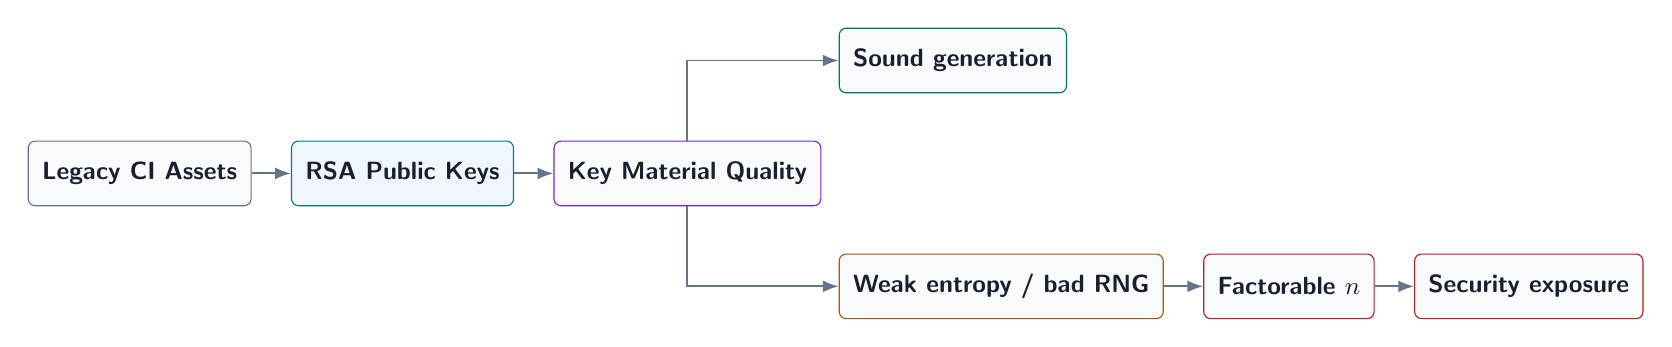
\begin{tikzpicture}[node distance=0.45cm and 0.5cm]
  \node[boxmut] (a) {Legacy CI Assets};
  \node[boxcyan, right=of a] (b) {RSA Public Keys};
  \node[boxvio, right=of b] (c) {Key Material Quality};
  \node[boxok, above right=0.6cm and 0.22cm of c] (e) {Sound generation};
  \node[boxamb, below right=0.6cm and 0.22cm of c] (d) {Weak entropy / bad RNG};
  \node[boxred, right=of d] (f) {Factorable $n$};
  \node[boxred, right=of f] (g) {Security exposure};
  \draw[arr] (a)--(b); \draw[arr] (b)--(c);
  \draw[arr] (c)|-(e); \draw[arr] (c)|-(d);
  \draw[arr] (d)--(f); \draw[arr] (f)--(g);
\end{tikzpicture}
\vspace{\fill}
\begin{minipage}[t]{0.32\textwidth}
\fcolorbox{cyan}{pane}{\begin{minipage}[t]{0.94\textwidth}\vspace{5pt}
{\large\bfseries\color{cyan}Silent mathematical failure}\\[0.3em]
\begin{itemize}\normalsize
  \item RSA rests on hardness of factoring $n=p\times q$
  \item Small/structured factors can make $n$ breakable via ECM
  \item Device may still encrypt/decrypt normally
  \item Weakness is mathematical, not a visible outage
\end{itemize}
\vspace{3pt}\end{minipage}}
\end{minipage}\hfill
\begin{minipage}[t]{0.32\textwidth}
\fcolorbox{amber}{pane}{\begin{minipage}[t]{0.94\textwidth}\vspace{5pt}
{\large\bfseries\color{amber}Legacy inventory pain}\\[0.3em]
\begin{itemize}\normalsize
  \item Years of certs, device keys, VPN/gateway keys
  \item Generation history often unknown
  \item Manual review cannot scale
  \item Bit-length alone misses weak primes inside ``large'' $n$
\end{itemize}
\vspace{3pt}\end{minipage}}
\end{minipage}\hfill
\begin{minipage}[t]{0.32\textwidth}
\fcolorbox{violet}{pane}{\begin{minipage}[t]{0.94\textwidth}\vspace{5pt}
{\large\bfseries\color{violet}What auditors need}\\[0.3em]
\begin{itemize}\normalsize
  \item Structural + mathematical checks
  \item Concrete evidence when a factor appears
  \item Clear tiered labels for findings
  \item Exportable reports for remediation
\end{itemize}
\vspace{3pt}\end{minipage}}
\end{minipage}
\vspace{\fill}
\end{slidepage}

%% 3 GAP
\begin{slidepage}
\slidetitle{From Key Inventory to Mathematical Assurance}
\begin{minipage}[t]{0.48\textwidth}
\fcolorbox{crit}{pane}{\begin{minipage}[t]{0.95\textwidth}\vspace{6pt}
{\large\bfseries\color{crit}Typical existing practice}\\[0.35em]
\begin{enumerate}\normalsize
  \item Collect keys into inventories / spreadsheets
  \item Check bit length (1024 / 2048 / 4096)
  \item Check public exponent / basic config flags
  \item Mark ``OK'' if length looks acceptable
\end{enumerate}
\vspace{0.3em}
\textcolor{crit}{\normalsize\textbf{Gap:} length $\neq$ mathematical strength. Weak primes can hide inside a large-looking modulus.}
\vspace{4pt}\end{minipage}}
\end{minipage}\hfill
\begin{minipage}[t]{0.48\textwidth}
\fcolorbox{cyan}{pane}{\begin{minipage}[t]{0.95\textwidth}\vspace{6pt}
{\large\bfseries\color{cyan}RSA-SHIELD approach}\\[0.35em]
\begin{enumerate}\normalsize
  \item Parse \& validate RSA public key / modulus
  \item Structural and parameter analysis
  \item Budgeted Lenstra ECM factorization attempts
  \item Evidence-tiered risk class + JSON/PDF report
\end{enumerate}
\vspace{0.3em}
\textcolor{cyan}{\normalsize\textbf{Value:} established math becomes a practical audit workflow with exportable evidence.}
\vspace{4pt}\end{minipage}}
\end{minipage}
\vspace{\fill}
{\normalsize\bfseries End-to-end audit pipeline}\\[0.35em]
\centering

\begin{tikzpicture}[node distance=0.28cm]
  \node[boxcyan] (a) {Key Input};
  \node[boxcyan, right=of a] (b) {Parse};
  \node[boxcyan, right=of b] (c) {Extract $n,e$};
  \node[boxvio, right=of c] (d) {Struct.\ Analysis};
  \node[boxvio, right=of d] (e) {ECM Probe};
  \node[boxamb, right=of e] (f) {Evidence};
  \node[boxcyan, right=of f] (g) {Risk Class};
  \node[boxok, right=of g] (h) {JSON/PDF Report};
  \draw[arr] (a)--(b); \draw[arr] (b)--(c); \draw[arr] (c)--(d);
  \draw[arr] (d)--(e); \draw[arr] (e)--(f); \draw[arr] (f)--(g); \draw[arr] (g)--(h);
\end{tikzpicture}
\vspace{\fill}
\fcolorbox{violet}{pane}{\begin{minipage}{\dimexpr\textwidth-12pt\relax}\vspace{6pt}
{\normalsize\color{body}\textbf{Positioning (Team Aegis):} We did \textbf{not} invent RSA or ECM. RSA-SHIELD is a security auditing platform that operationalizes known algorithms for authorized assessment at \textbf{Bennett University} under \textbf{Dr.\ Sachin Choudhary}.\\[0.3em]
\textbf{Tiers:} Factor Found (math) $\cdot$ Suspicious (heuristic) $\cdot$ Inconclusive (no factor in budget) $\cdot$ No weakness by configured checks.}
\vspace{4pt}\end{minipage}}
\vspace{\fill}
\end{slidepage}

%% 4 ENGINE
\begin{slidepage}
\slidetitle{Inside the Audit Engine --- How RSA-SHIELD Works}
\begin{minipage}[t]{0.52\textwidth}
\fcolorbox{cyan}{pane2}{\begin{minipage}{0.95\textwidth}\vspace{6pt}\centering
{\Large\bfseries $n = p \times q$}\\[0.3em]
{\normalsize\color{body}Recovering a non-trivial factor of $n$ compromises the RSA modulus and enables private-key recovery.}
\vspace{4pt}\end{minipage}}
\vspace{0.4em}
{\large\bfseries\color{cyan}Detailed processing steps}
\begin{enumerate}\normalsize
  \item \textbf{Ingest} PEM/DER public key or raw modulus integer
  \item \textbf{Validate} encoding, structure, required fields
  \item \textbf{Extract} public modulus $n$ and exponent $e$
  \item \textbf{Preliminary checks} bit-length, unusual $e$, trivial divisibility
  \item \textbf{ECM campaign} configurable curves, bounds, time budget
  \item \textbf{Factor handling} store non-trivial factors if found
  \item \textbf{Exposure mapping} evidence $\rightarrow$ severity class
  \item \textbf{Persist \& report} history + JSON/PDF export
\end{enumerate}
\end{minipage}\hfill
\begin{minipage}[t]{0.44\textwidth}
\centering
{\normalsize\color{muted}\textbf{Audit lifecycle}}\\[0.25em]
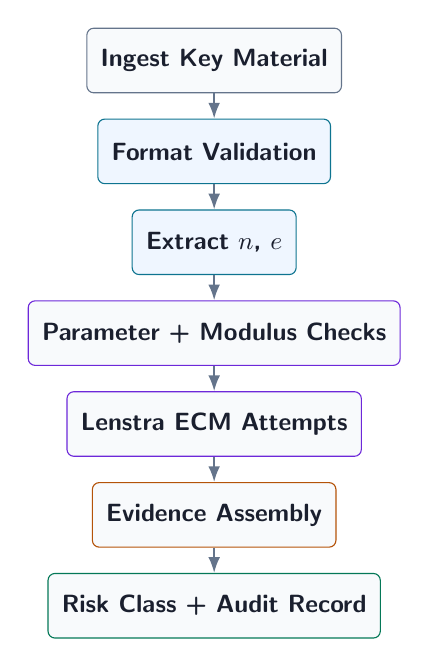
\begin{tikzpicture}[node distance=0.32cm]
  \node[boxmut] (a) {Ingest Key Material};
  \node[boxcyan, below=of a] (b) {Format Validation};
  \node[boxcyan, below=of b] (c) {Extract $n$, $e$};
  \node[boxvio, below=of c] (d) {Parameter + Modulus Checks};
  \node[boxvio, below=of d] (e) {Lenstra ECM Attempts};
  \node[boxamb, below=of e] (f) {Evidence Assembly};
  \node[boxok, below=of f] (g) {Risk Class + Audit Record};
  \draw[arr] (a)--(b); \draw[arr] (b)--(c); \draw[arr] (c)--(d);
  \draw[arr] (d)--(e); \draw[arr] (e)--(f); \draw[arr] (f)--(g);
\end{tikzpicture}
\vspace{\fill}
\fcolorbox{violet}{pane}{\begin{minipage}{0.95\textwidth}\vspace{5pt}
{\normalsize\color{body}Orchestrator coordinates \textbf{Parser}, \textbf{Key Analyzer}, \textbf{ECM Engine}, \textbf{Risk Engine}, and \textbf{Report Generator} as separate modules with timeouts and audit logging.}
\vspace{3pt}\end{minipage}}
\end{minipage}
\vspace{\fill}
\end{slidepage}

%% 5 ECM
\begin{slidepage}
\slidetitle{Why Lenstra's Elliptic Curve Method (ECM)?}
\begin{minipage}[t]{0.50\textwidth}
{\normalsize\color{body}Lenstra ECM is a classic integer-factorization algorithm. It is especially effective when a large composite has a \textbf{relatively small} prime factor---a failure mode that can appear in poorly generated RSA moduli used by legacy devices.}
\vspace{\fill}
{\large\bfseries\color{cyan}Auditor's conceptual view}
\begin{itemize}\normalsize
  \item Sample random elliptic curves modulo $n$
  \item Curve arithmetic can fail when a factor of $n$ divides a bad denominator
  \item A non-trivial $\gcd$ with $n$ reveals a factor = strong evidence
  \item No factor within budget $\Rightarrow$ \textbf{inconclusive}, not ``proven secure''
\end{itemize}
\vspace{\fill}
\fcolorbox{amber}{pane}{\begin{minipage}{0.95\textwidth}\vspace{5pt}
{\normalsize\color{amber}\textbf{Honest limit:} ECM does not instantly factor properly generated modern RSA (e.g.\ strong 2048-bit primes). RSA-SHIELD uses ECM as a \textbf{weakness probe}, not a universal RSA break.}
\vspace{3pt}\end{minipage}}
\end{minipage}\hfill
\begin{minipage}[t]{0.46\textwidth}
\centering
{\normalsize\color{muted}\textbf{ECM audit workflow}}\\[0.25em]
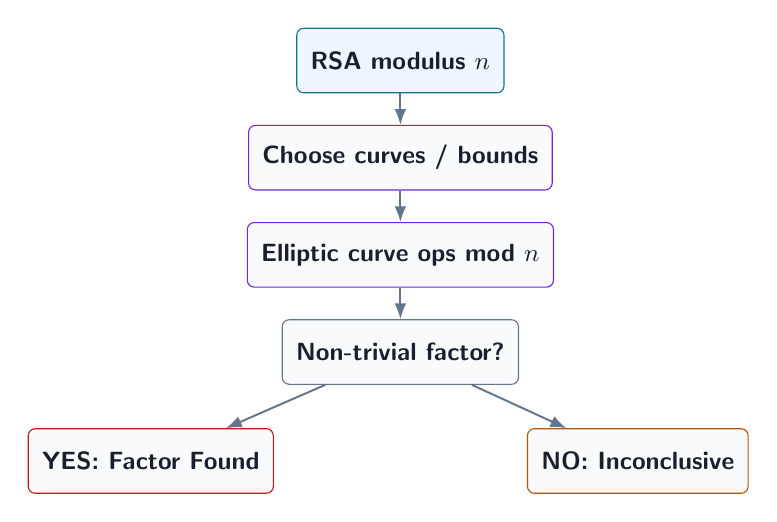
\begin{tikzpicture}[node distance=0.4cm]
  \node[boxcyan] (n) {RSA modulus $n$};
  \node[boxvio, below=of n] (s) {Choose curves / bounds};
  \node[boxvio, below=of s] (e) {Elliptic curve ops mod $n$};
  \node[boxmut, below=of e] (q) {Non-trivial factor?};
  \node[boxred, below left=0.55cm and 0.1cm of q] (y) {YES: Factor Found};
  \node[boxamb, below right=0.55cm and 0.1cm of q] (x) {NO: Inconclusive};
  \draw[arr] (n)--(s); \draw[arr] (s)--(e); \draw[arr] (e)--(q);
  \draw[arr] (q)--(y); \draw[arr] (q)--(x);
\end{tikzpicture}
\vspace{\fill}
\fcolorbox{violet}{pane}{\begin{minipage}{0.95\textwidth}\vspace{5pt}
{\normalsize\bfseries\color{violet}Why this fits legacy CI}\\[0.25em]
{\normalsize\color{body}Old embedded RNGs and rushed key generation can leave small factors. Finding one factor proves the modulus unsafe and supports immediate key rotation---with evidence, not guesswork.}
\vspace{3pt}\end{minipage}}
\end{minipage}
\vspace{\fill}
\end{slidepage}

%% 6 ARCHITECTURE
\begin{slidepage}
\slidetitle{RSA-SHIELD System Architecture}
\centering
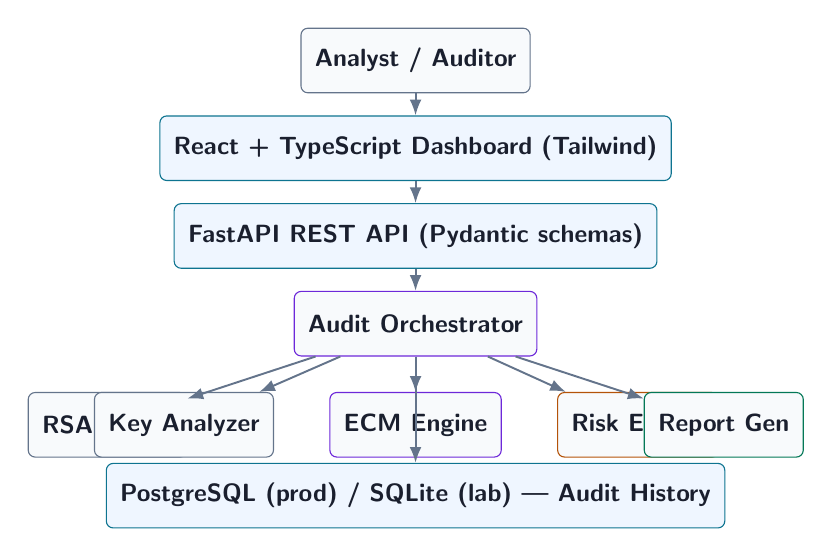
\begin{tikzpicture}[node distance=0.28cm and 0.38cm]
  \node[boxmut] (u) {Analyst / Auditor};
  \node[boxcyan, below=of u] (fe) {React + TypeScript Dashboard (Tailwind)};
  \node[boxcyan, below=of fe] (api) {FastAPI REST API (Pydantic schemas)};
  \node[boxvio, below=of api] (orch) {Audit Orchestrator};
  \node[boxmut, below left=0.45cm and 1.35cm of orch] (p) {RSA Parser};
  \node[boxmut, below left=0.45cm and 0.25cm of orch] (k) {Key Analyzer};
  \node[boxvio, below=0.45cm of orch] (ecm) {ECM Engine};
  \node[boxamb, below right=0.45cm and 0.25cm of orch] (r) {Risk Engine};
  \node[boxok, below right=0.45cm and 1.35cm of orch] (rep) {Report Gen};
  \node[boxcyan, below=1.35cm of orch] (db) {PostgreSQL (prod) / SQLite (lab) --- Audit History};
  \draw[arr] (u)--(fe); \draw[arr] (fe)--(api); \draw[arr] (api)--(orch);
  \draw[arr] (orch)--(p); \draw[arr] (orch)--(k); \draw[arr] (orch)--(ecm);
  \draw[arr] (orch)--(r); \draw[arr] (orch)--(rep); \draw[arr] (orch)--(db);
\end{tikzpicture}
\vspace{\fill}
\begin{minipage}[t]{0.32\textwidth}
\fcolorbox{cyan}{pane}{\begin{minipage}{0.94\textwidth}\vspace{5pt}
{\large\bfseries\color{cyan}Frontend}\\[0.25em]
\begin{itemize}\normalsize
  \item Key upload \& batch queue
  \item Status / severity badges
  \item Pipeline visualizations
  \item History + report download
\end{itemize}
\vspace{3pt}\end{minipage}}
\end{minipage}\hfill
\begin{minipage}[t]{0.32\textwidth}
\fcolorbox{violet}{pane}{\begin{minipage}{0.94\textwidth}\vspace{5pt}
{\large\bfseries\color{violet}Backend}\\[0.25em]
\begin{itemize}\normalsize
  \item Validated API contracts
  \item ECM job timeouts/budgets
  \item Evidence artifact storage
  \item JSON + PDF assembly
\end{itemize}
\vspace{3pt}\end{minipage}}
\end{minipage}\hfill
\begin{minipage}[t]{0.32\textwidth}
\fcolorbox{ok}{pane}{\begin{minipage}{0.94\textwidth}\vspace{5pt}
{\large\bfseries\color{ok}Deployment}\\[0.25em]
\begin{itemize}\normalsize
  \item Dockerized services
  \item SQLite demos; Postgres labs
  \item GitHub CI with Pytest
  \item Environment-based config
\end{itemize}
\vspace{3pt}\end{minipage}}
\end{minipage}
\vspace{\fill}
\end{slidepage}

%% 7 ANALYSIS
\begin{slidepage}
\slidetitle{Layered Analysis Engine and Authorized Audit Scenario}
\begin{minipage}[t]{0.48\textwidth}
{\large\bfseries\color{cyan}Six analysis layers}
\begin{enumerate}\normalsize
  \item \textbf{Format \& parameter validation} --- PEM/DER sanity
  \item \textbf{RSA parameter analysis} --- $e$, size, anomalies
  \item \textbf{Modulus characteristics} --- trivial factor screens
  \item \textbf{ECM factorization attempt} --- budgeted math probe
  \item \textbf{Evidence-based risk class} --- proof vs heuristic
  \item \textbf{Audit report} --- human + machine readable
\end{enumerate}
\vspace{\fill}
{\normalsize\color{violet}\textbf{Principle:} mathematical evidence (factor found) is never mixed with soft warnings without explicit labeling.}
\vspace{\fill}
\fcolorbox{crit}{pane}{\begin{minipage}{0.95\textwidth}\vspace{5pt}
{\normalsize\bfseries Mock dashboard (illustrative)}\\[0.3em]
{\normalsize
\begin{tabular}{@{}ll@{}}
Key ID & \texttt{LEGACY-SCADA-0042}\\[0.15em]
Modulus & 1024-bit\\[0.15em]
Exponent & $e=65537$\\[0.15em]
ECM status & Factor discovered\\[0.15em]
Severity & CRITICAL\\[0.15em]
Action & Recommend key rotation\\
\end{tabular}}
\vspace{3pt}\end{minipage}}
\end{minipage}\hfill
\begin{minipage}[t]{0.48\textwidth}
\centering
{\normalsize\color{muted}\textbf{Authorized scenario (owner consent / lab keys)}}\\[0.3em]
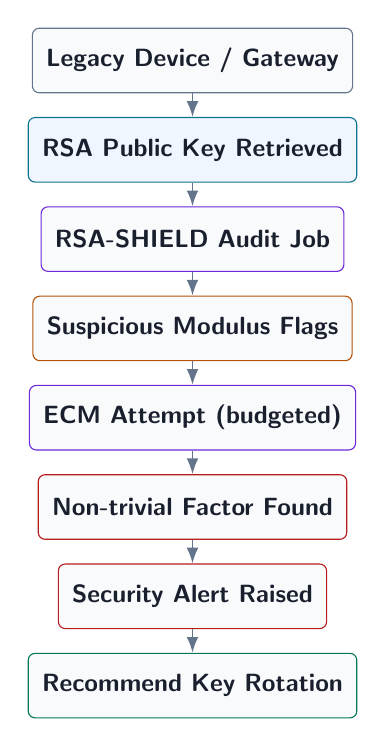
\begin{tikzpicture}[node distance=0.3cm]
  \node[boxmut] (a) {Legacy Device / Gateway};
  \node[boxcyan, below=of a] (b) {RSA Public Key Retrieved};
  \node[boxvio, below=of b] (c) {RSA-SHIELD Audit Job};
  \node[boxamb, below=of c] (d) {Suspicious Modulus Flags};
  \node[boxvio, below=of d] (e) {ECM Attempt (budgeted)};
  \node[boxred, below=of e] (f) {Non-trivial Factor Found};
  \node[boxred, below=of f] (g) {Security Alert Raised};
  \node[boxok, below=of g] (h) {Recommend Key Rotation};
  \draw[arr] (a)--(b); \draw[arr] (b)--(c); \draw[arr] (c)--(d);
  \draw[arr] (d)--(e); \draw[arr] (e)--(f); \draw[arr] (f)--(g); \draw[arr] (g)--(h);
\end{tikzpicture}
\vspace{\fill}
{\normalsize\color{muted}Factor-discovery claims apply only when demonstrated on authorized or intentionally weak test keys.}
\end{minipage}
\vspace{\fill}
\end{slidepage}

%% 8 STACK
\begin{slidepage}
\slidetitle{Technology Stack, Product Features, Evaluation Plan}
\begin{minipage}[t]{0.33\textwidth}
\fcolorbox{cyan}{pane}{\begin{minipage}{0.94\textwidth}\vspace{5pt}
{\large\bfseries\color{cyan}Technology stack}\\[0.3em]
{\normalsize
\begin{tabular}{@{}ll@{}}
\textbf{UI} & React, TS, Tailwind, Vite\\
 & React Flow / Recharts\\[0.15em]
\textbf{API} & Python, FastAPI, Pydantic\\[0.15em]
\textbf{Engine} & RSA math, modular arith.\\
 & Lenstra ECM modules\\[0.15em]
\textbf{Data} & PostgreSQL / SQLite\\[0.15em]
\textbf{DevOps} & Docker, Git, GitHub\\[0.15em]
\textbf{Test} & Pytest unit+integration\\
\end{tabular}}
\vspace{3pt}\end{minipage}}
\end{minipage}\hfill
\begin{minipage}[t]{0.33\textwidth}
\fcolorbox{violet}{pane}{\begin{minipage}{0.94\textwidth}\vspace{5pt}
{\large\bfseries\color{violet}Product features}\\[0.25em]
\begin{itemize}\normalsize
  \item RSA key / modulus upload
  \item Batch key auditing
  \item Modulus \& parameter analysis
  \item Configurable ECM attempts
  \item Audit history \& evidence store
  \item Risk classification badges
  \item JSON + PDF reports
  \item API for workflows
  \item Audit simulation mode
  \item Interactive visualizations
\end{itemize}
\vspace{3pt}\end{minipage}}
\end{minipage}\hfill
\begin{minipage}[t]{0.30\textwidth}
\fcolorbox{amber}{pane}{\begin{minipage}{0.94\textwidth}\vspace{5pt}
{\large\bfseries\color{amber}Evaluation metrics}\\[0.25em]
\begin{itemize}\normalsize
  \item Parse success rate
  \item Audit latency
  \item ECM wall-clock time
  \item Detection on weak lab keys
  \item Heuristic FP rate
  \item Batch throughput
  \item CPU/memory use
\end{itemize}
\vspace{0.35em}
\centering\textbf{Prototype Benchmark}\\[0.15em]
\normalsize To Be Measured\\--- no fabricated numbers ---
\vspace{3pt}\end{minipage}}
\end{minipage}
\vspace{\fill}
\fcolorbox{cyan}{pane}{\begin{minipage}{\dimexpr\textwidth-12pt\relax}\vspace{6pt}
{\normalsize\color{body}\textbf{Evaluation discipline:} detection rates are reported only for \textbf{intentionally weak test keys} under authorized lab conditions at Bennett University. ECM failure on a strong key is recorded as \textbf{inconclusive}, never as a security proof.}
\vspace{4pt}\end{minipage}}
\vspace{\fill}
\end{slidepage}

%% 9 LIMITS
\begin{slidepage}
\slidetitle{What RSA-SHIELD Does --- and Does Not --- Claim}
\begin{minipage}[t]{0.48\textwidth}
\fcolorbox{cyan}{pane}{\begin{minipage}{0.95\textwidth}\vspace{6pt}
{\large\bfseries\color{cyan}What Team Aegis claims}\\[0.4em]
\begin{itemize}\normalsize
  \item Accepts/parses RSA public keys and moduli
  \item Performs structural and parameter analysis
  \item Runs budgeted Lenstra ECM as a weakness probe
  \item Treats a discovered factor as \textbf{hard evidence}
  \item Separates evidence from heuristic warnings
  \item Produces understandable JSON/PDF assessments
  \item Supports authorized inventory audit workflows
\end{itemize}
\vspace{0.35em}
\textcolor{cyan}{\normalsize\textbf{Goal:} help owners find weak legacy keys before adversaries do.}
\vspace{4pt}\end{minipage}}
\end{minipage}\hfill
\begin{minipage}[t]{0.48\textwidth}
\fcolorbox{crit}{pane}{\begin{minipage}{0.95\textwidth}\vspace{6pt}
{\large\bfseries\color{crit}What we explicitly do not claim}\\[0.4em]
\begin{itemize}\normalsize
  \item ECM is not a magic attack on modern strong RSA
  \item No factor found $\neq$ proof the key is secure
  \item Tool is an auditing aid, not a formal security proof
  \item Production needs specialist cryptographic review
  \item Only \textbf{authorized} keys/infrastructure may be audited
  \item We did not invent RSA, ECM, or a new cipher
\end{itemize}
\vspace{0.35em}
\textcolor{crit}{\normalsize\textbf{Credibility} comes from precise, responsible claims.}
\vspace{4pt}\end{minipage}}
\end{minipage}
\vspace{\fill}
\fcolorbox{violet}{pane}{\begin{minipage}{\dimexpr\textwidth-12pt\relax}\vspace{6pt}
{\normalsize\color{body}This strengthens the project for evaluators: Team Aegis understands both the \textbf{power} and the \textbf{limits} of factorization-based auditing. Responsible framing is part of the engineering contribution under mentorship of \textbf{Dr.\ Sachin Choudhary} at \textbf{Bennett University}.}
\vspace{4pt}\end{minipage}}
\vspace{\fill}
\end{slidepage}

%% 10 FUTURE
\begin{slidepage}
\slidetitle{From RSA Auditor to Cryptographic Asset Intelligence}
{\normalsize\color{body}Near-term RSA-SHIELD focuses on single-key and batch modulus auditing. The roadmap expands toward continuous cryptographic asset intelligence for enterprises and critical-infrastructure operators.}
\vspace{\fill}
\centering
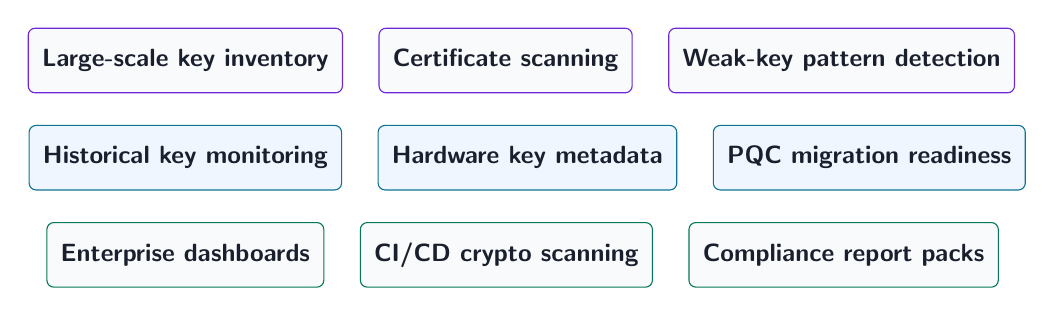
\begin{tikzpicture}[node distance=0.4cm and 0.45cm]
  \node[boxvio] (a) {Large-scale key inventory};
  \node[boxvio, right=of a] (b) {Certificate scanning};
  \node[boxvio, right=of b] (c) {Weak-key pattern detection};
  \node[boxcyan, below=of a] (d) {Historical key monitoring};
  \node[boxcyan, right=of d] (e) {Hardware key metadata};
  \node[boxcyan, right=of e] (f) {PQC migration readiness};
  \node[boxok, below=of d] (g) {Enterprise dashboards};
  \node[boxok, right=of g] (h) {CI/CD crypto scanning};
  \node[boxok, right=of h] (i) {Compliance report packs};
\end{tikzpicture}
\vspace{\fill}
\begin{minipage}[t]{0.32\textwidth}
\fcolorbox{violet}{pane}{\begin{minipage}{0.94\textwidth}\vspace{5pt}
{\normalsize\bfseries\color{violet}Inventory scale}\\[0.2em]
{\normalsize\color{body}Fleet-wide discovery of RSA assets across devices, certificates, and services.}
\vspace{3pt}\end{minipage}}
\end{minipage}\hfill
\begin{minipage}[t]{0.32\textwidth}
\fcolorbox{cyan}{pane}{\begin{minipage}{0.94\textwidth}\vspace{5pt}
{\normalsize\bfseries\color{cyan}Continuous assurance}\\[0.2em]
{\normalsize\color{body}Track key health over time; alert when new weak patterns appear.}
\vspace{3pt}\end{minipage}}
\end{minipage}\hfill
\begin{minipage}[t]{0.32\textwidth}
\fcolorbox{ok}{pane}{\begin{minipage}{0.94\textwidth}\vspace{5pt}
{\normalsize\bfseries\color{ok}Enterprise readiness}\\[0.2em]
{\normalsize\color{body}Dashboards, CI gates, and compliance packs for operators.}
\vspace{3pt}\end{minipage}}
\end{minipage}
\vspace{\fill}
\fcolorbox{cyan}{pane2}{\begin{minipage}{\dimexpr\textwidth-12pt\relax}\vspace{8pt}\centering
{\LARGE\bfseries\color{cyan}Know Your Keys. Prove Their Strength.}\\[0.5em]
{\Large\bfseries Team Aegis}\\[0.35em]
{\normalsize
Nishant Agarwal (\texttt{S24CSEU1512}) \quad
Adarsh Agrahari (\texttt{S24CSEU1187}) \quad
Shubh Jadiya (\texttt{S24CSEU0530})}\\[0.35em]
{\normalsize Mentor: \textbf{Dr.\ Sachin Choudhary} \quad Institution: \textbf{Bennett University}}\\[0.25em]
{\normalsize\color{cyan}GitHub: \texttt{https://github.com/team-aegis/rsa-shield}}
\vspace{6pt}\end{minipage}}
\vspace{\fill}
\end{slidepage}

\end{document}
